\documentclass[12pt]{beamer}

\usetheme{CambridgeUS}
\usepackage[utf8]{inputenc}
\usepackage{lmodern}
\usepackage{listings}
\usepackage{graphicx}


\begin{document}

\frame {
    \maketitle
}

% Begin Joan Vilà

\frame {
    \frametitle{Instalación: tiempo y problemas}
    \begin{itemize}
        \item {Windows 10}
        \item {Ubuntu}
        \item {Mac OS}
    \end{itemize}
}

\frame {
    \frametitle{Instalación de Windows}
    \begin{enumerate}
        \item {Descargar la ISO (v10 3,71GB)}
        \item {Grabar en un CD o USB}
        \item {Reiniciar arrancando desde CD o USB}
        \item {Instalar medinte boton de siguiente}
        \item {Conseguir o tener una licencia válida y demostrarlo}
    \end{enumerate}
}

\frame {
    \frametitle{Instalación de Ubuntu}
    \begin{enumerate}
        \item {Descargar la ISO (v16.04 1,51GB)}
        \item {Grabar en un CD o USB}
        \item {Reiniciar arrancando desde CD o USB}
        \item {Instalar medinte boton de siguiente}
    \end{enumerate}
}

\frame {
    \frametitle{Instalación de MacOS}
    \begin{enumerate}
        \item {Reiniciar en modo recuperación}
        \item {Seleccionar reinstalar el SO}
        \item {Esperar (vSierra 4,86GB)}
    \end{enumerate}
}

\frame {
    \frametitle{Ventajas de cada uno}
    \begin{itemize}
        \item {Windows: ???}
        \item {Ubuntu: Gratis, posibilidad de instalarlo al lado de otros SO}
        \item {MacOS: Facil, nivel usuaro bajo}
    \end{itemize}
}

\frame {
    \frametitle{Desventajas de cada uno}
    \begin{itemize}
        \item {Windows: Grabar la ISO y el precio/licencia}
        \item {Ubuntu: Grabar la ISO}
        \item {MacOS: Tiempo de descarga}
    \end{itemize}
}

\frame {
    \frametitle{Aplicaciones disponibles y coste}
    \textbf{Comparación entre Windows Store, ubuntu sofware center y mac AppStore}
}

\frame {
    \frametitle{Windows Store}
    \begin{itemize}
        \item {669.000 apps para moviles, ordenadores y tabletas}
        \item {Ojo! Sólo aplicaciones universales}
    \end{itemize}
}

\frame {
    \frametitle{Ubuntu Software Center}
    \begin{itemize}
        \item {Número de apps desconocido}
        \item {El número depende de las fuentes en las que se confie}
        \item {Posibilidad de añadir y quitar fuentes a gusto}
    \end{itemize}
}

\frame {
    \frametitle{Mac App Store}
    \begin{itemize}
        \item {31.191 apps disponibles para Mac}
        \item {Estricto filtro para colgar una app}
        \item {Travas para utilizar apps de terceros}
    \end{itemize}
}

\frame {
    \frametitle{Comparando las alternativas}
    \begin{itemize}
        \item {Windows: necesidad de buscar la vida por internet}
        \item {Mac: utilizar Homebrew como fuente de software y buscar la vida por internet}
        \item {Ubuntu: Difícil compatibilidad con software privativo de las otras plataformas}
    \end{itemize}
}

\frame {
    \frametitle{Comparativa de precios}
    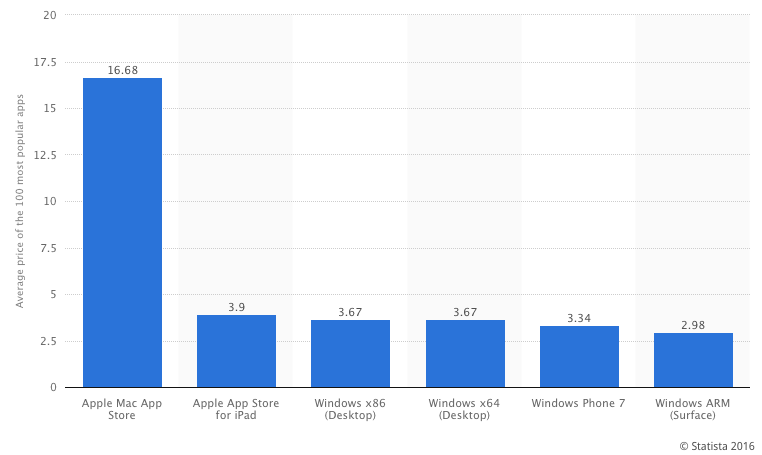
\includegraphics[width=\textwidth]{PriceComparison.png}
}

\frame {
    \frametitle{Reflexión de problemas vistos hasta el momento}
    \begin{itemize}
        \item {Windows: Software propenso a virus y con problemas de privacidad}
        \item {Mac: Hacks como Homebrew para acceder a fuentes de software y problemas de privacidad}
        \item {Ubuntu: No es posible utilizar sofware popular de Microsoft, Adobe... (wine)}
    \end{itemize}
}

% End Joan Vilà
% Begin Sergi Soriano

\frame {
    \frametitle{Velocidad de arranque / ejecución de aplicaciones / copias}
    \textbf{Sergi Soriano}
}

% End Sergi Soriano
% Begin Miquel Xamani

\frame {
    \frametitle{Uso de recursos del sistema (usuario y/o servidor)}
    \textbf{Miquel Xamani}
}

% End Miquel Xamani
% Begin Arnau Garcia

\frame {
    \frametitle{Comparativa de tiempos/recursos para una aplicación en el mismo PC bajo distintos SO}
    \framesubtitle{Introducció}
    \begin{itemize}
    \item {Interacció entre els components del sistema operatiu i el temps d'execució segueix sent en part un misteri}
    \end{itemize}
    \begin{enumerate}
    \item{Fallades de la memòria de traducció (TLB)}
    \item{Interrupcions}
    \item{Events asíncrons}
    \end{enumerate}
    \begin{itemize}
    \item{Poden \textbf{afectar el rendiment} dels SO}
    \end{itemize}
}
\frame {
    \frametitle{Comparativa de tiempos/recursos para una aplicación en el mismo PC bajo distintos SO}
    \framesubtitle{Introducció}
    \begin{itemize}
    \item {\textbf{Soroll}: interferència del sistema operatiu}
    \item{Important intentar definir/interpretar el que es considera soroll:}
    \end{itemize}
    \begin{center}
    \large{\emph{"Col·lecció d'activitats de fons que involuntàriament interrumpeixen el progrés de l'aplicació principal.”}}
    \end{center}
}
\frame {
    \frametitle{Comparativa de tiempos/recursos para una aplicación en el mismo PC bajo distintos SO}
    \framesubtitle{Simulació 1 - Factorial}
    \begin{itemize}
    \item {Sistemes operatius:}
	\begin{itemize}
	\item\textbf{openSUSE 13.2 (Harlequin) (64 bits)}
    	\item\textbf{Windows 7 ENTERPRISE (64 bits)}
    	\end{itemize}
    \item {Medició:}
	\begin{itemize}
	\item\textbf{Factorial de 10}
    	\end{itemize}
    \item {Processador:}
	\begin{itemize}
	\item\textbf{Intel(R) Core(TM) i5-3470 CPU @ 3.20GHz - 64 bits}
    	\end{itemize}
    \item {Memòria RAM:}
	\begin{itemize}
	\item\textbf{8 GB}
    	\end{itemize}
    \item {Nom de l'equip:}
	\begin{itemize}
	\item\textbf{c6s301pc42}
    	\end{itemize}
    \item {Domini:}
	\begin{itemize}
	\item\textbf{FIBSMB}
    	\end{itemize}
    \end{itemize}
}
\frame {
    \frametitle{Comparativa de tiempos/recursos para una aplicación en el mismo PC bajo distintos SO}
    \framesubtitle{Simulació 1 - Factorial}
    \begin{itemize}
    \item\textbf{openSUSE}
   % \begin{lstlisting}[language=bash,caption={bash version}]#!/bin/bashecho "Hello, world!"\end{lstlisting}
    \item\textbf{!/bin/bash
	START="$(($(date +%s%N)/1000000))"
	cd /home/Desktop/
	./factorial.out
	END="$(($(date +%s%N)/1000000))" 
	TOTAL=$(($END-$START))
	echo "END: "$END "START: "$START "TOTAL: "$TOTAL}
    \end{itemize}
}
\frame {
    \frametitle{Comparativa de tiempos/recursos para una aplicación en el mismo PC bajo distintos SO}
    \framesubtitle{Simulació 1 - Factorial}

  \begin{tabular}{cl}  
         \begin{tabular}{c}
           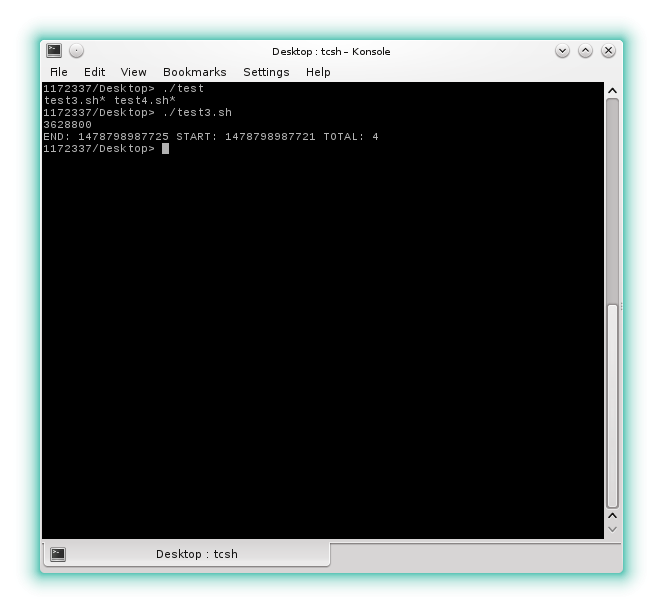
\includegraphics[height=8cm, width=7cm]{factorial_open_suse.png}
           \end{tabular}
           & \begin{tabular}{l}
             \parbox{0.5\linewidth}{
	     \begin{itemize}
             \item\textbf{openSUSE}
	     \item\textbf{4 Mil·lisegons}
	     \end{itemize}}
         \end{tabular}  \\
\end{tabular}
}
\frame {
    \frametitle{Comparativa de tiempos/recursos para una aplicación en el mismo PC bajo distintos SO}
    \framesubtitle{Simulació 1 - Factorial}
    \begin{itemize}
    \item\textbf{Windows}
   % \begin{lstlisting}[language=bash,caption={bash version}]#!/bin/bashecho "Hello, world!"\end{lstlisting}
    \item\textbf{@ECHO OFF
SET START= %time% 
start /WAIT a.exe
SET END= %time% 
SET /a TOTAL = %END% - %START%
ECHO END:} %END% START: %START% TOTAL: %TOTAL%}
    \end{itemize}
}
\frame {
    \frametitle{Comparativa de tiempos/recursos para una aplicación en el mismo PC bajo distintos SO}
    \framesubtitle{Simulació 1 - Factorial}

  \begin{tabular}{cl}  
         \begin{tabular}{c}
           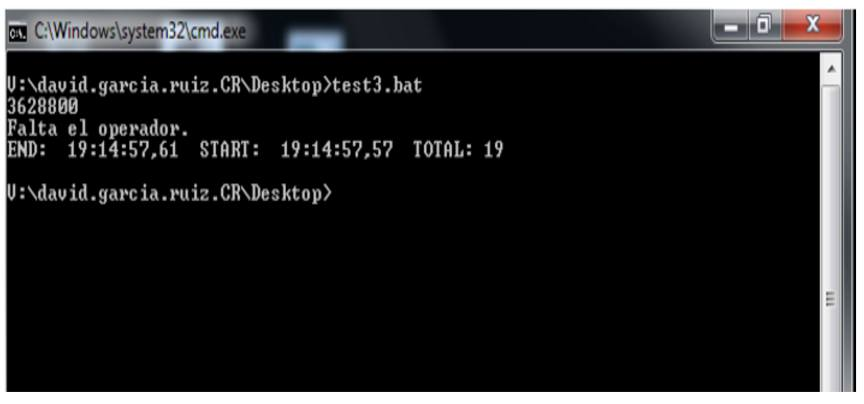
\includegraphics[height=4cm, width=7cm]{factorial_windows7.png}
           \end{tabular}
           & \begin{tabular}{l}
             \parbox{0.5\linewidth}{
	     \begin{itemize}
             \item\textbf{Windows 7}
	     \item\textbf{19 Mil·lisegons}
	     \end{itemize}}
         \end{tabular}  \\
\end{tabular}
}

\frame {
  \frametitle{Comparativa de tiempos/recursos para una aplicación en el mismo PC bajo distintos SO}
  \framesubtitle{Simulació 1 - Factorial}
  \begin{itemize}
  \item\textbf{openSUSE}
	  \begin{itemize}
	  \item{4 Mil·lisegons}
	  \end{itemize}
  \item\textbf{Windows 7}
	  \begin{itemize}
	  \item{19 Mil·lisegons}
	  \end{itemize}
   \end{itemize}
}

\frame {
    \frametitle{Comparativa de tiempos/recursos para una aplicación en el mismo PC bajo distintos SO}
    \framesubtitle{Simulació 2 - Linpack Benchmark}
    \begin{itemize}
    \item {Sistemes operatius:}
	\begin{itemize}
	\item\textbf{openSUSE 13.2 (Harlequin) (64 bits)}
    	\item\textbf{Windows 7 ENTERPRISE (64 bits)}
    	\end{itemize}
    \item {Medició:}
	\begin{itemize}
	\item\textbf{Linpack Benchmark}
    	\end{itemize}
    \item {Processador:}
	\begin{itemize}
	\item\textbf{Intel(R) Core(TM) i5-3470 CPU @ 3.20GHz - 64 bits}
    	\end{itemize}
    \item {Memòria RAM:}
	\begin{itemize}
	\item\textbf{8 GB}
    	\end{itemize}
    \item {Nom de l'equip:}
	\begin{itemize}
	\item\textbf{c6s301pc42}
    	\end{itemize}
    \item {Domini:}
	\begin{itemize}
	\item\textbf{FIBSMB}
    	\end{itemize}
    \end{itemize}
}
\frame {
    \frametitle{Comparativa de tiempos/recursos para una aplicación en el mismo PC bajo distintos SO}
    \framesubtitle{Simulació 2 - Linpack Benchmark}

  \begin{tabular}{cl}  
         \begin{tabular}{c}
           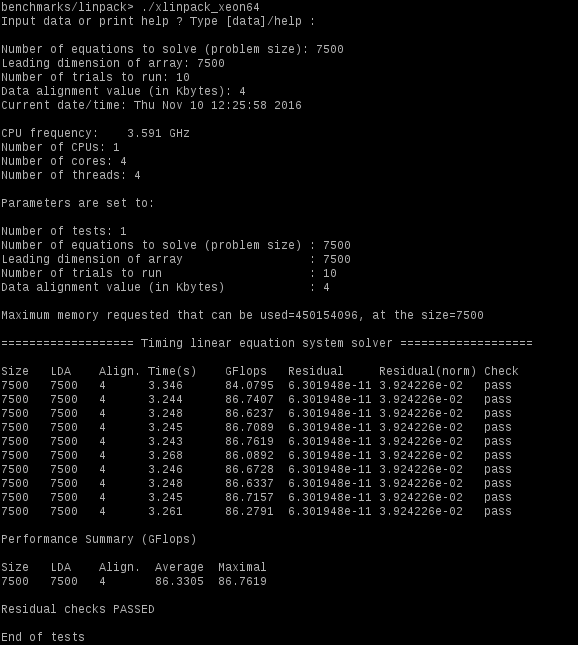
\includegraphics[height=7cm, width=6cm]{linpack_linux.png}
           \end{tabular}
           & \begin{tabular}{l}
             \parbox{0.5\linewidth}{
	     \begin{itemize}
             \item\textbf{openSUSE}
	     \item\textbf{Matrius 7500x7500}
	     \item\textbf{Promig 10 proves}
	     \end{itemize}}
         \end{tabular}  \\
\end{tabular}
}
\frame {
    \frametitle{Comparativa de tiempos/recursos para una aplicación en el mismo PC bajo distintos SO}
    \framesubtitle{Simulació 2 - Linpack Benchmark}

  \begin{tabular}{cl}  
         \begin{tabular}{c}
           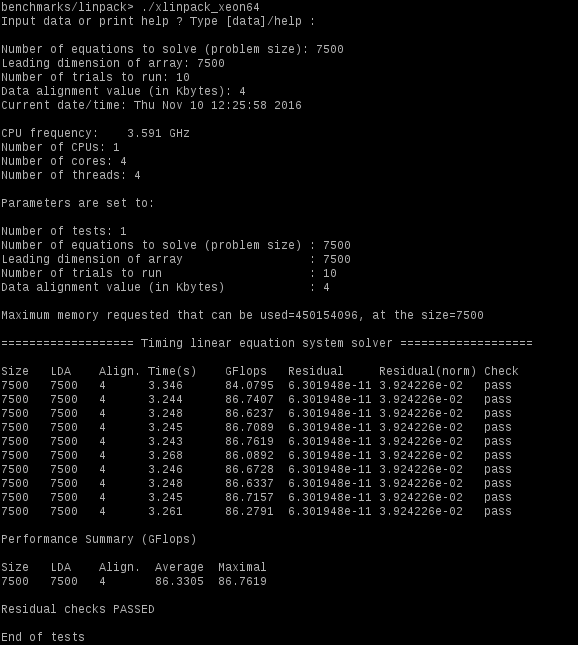
\includegraphics[height=7cm, width=6cm]{linpack_linux.png}
           \end{tabular}
           & \begin{tabular}{l}
             \parbox{0.5\linewidth}{
	     \begin{itemize}
             \item\textbf{openSUSE}
	     \item\textbf{Matrius 7500x7500}
	     \item\textbf{Promig 10 proves}
	     \item\textbf{86.3305 GFLOPS}
	     \end{itemize}}
         \end{tabular}  \\
\end{tabular}
}
\frame {
    \frametitle{Comparativa de tiempos/recursos para una aplicación en el mismo PC bajo distintos SO}
    \framesubtitle{Simulació 2 - Linpack Benchmark}

  \begin{center} 
    \begin{figure}
           \centering
           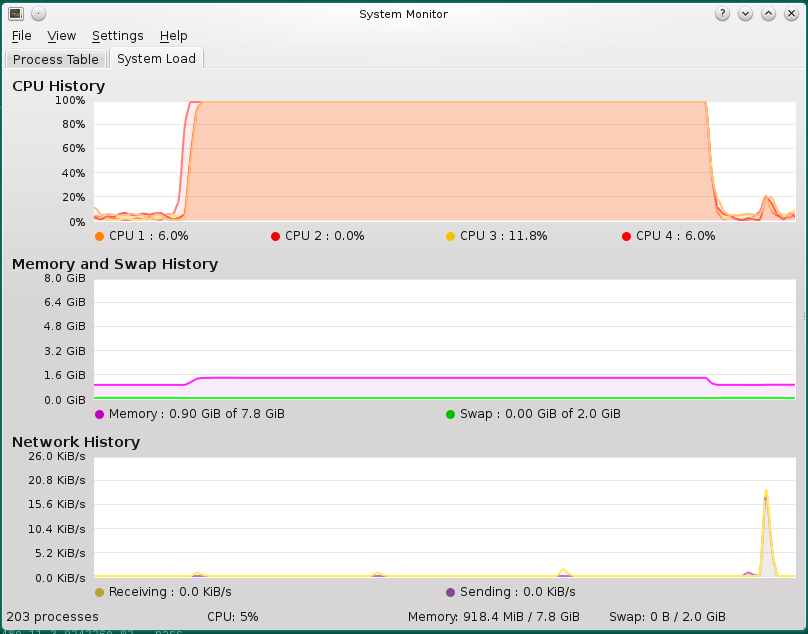
\includegraphics[height=6cm, width=8cm]{linuxmonitor.png}
           \caption{Monitor CPU Linux}
    \end{figure}
  \end{center}
  
}
\frame {
    \frametitle{Comparativa de tiempos/recursos para una aplicación en el mismo PC bajo distintos SO}
    \framesubtitle{Simulació 2 - Linpack Benchmark}

  \begin{tabular}{cl}  
         \begin{tabular}{c}
           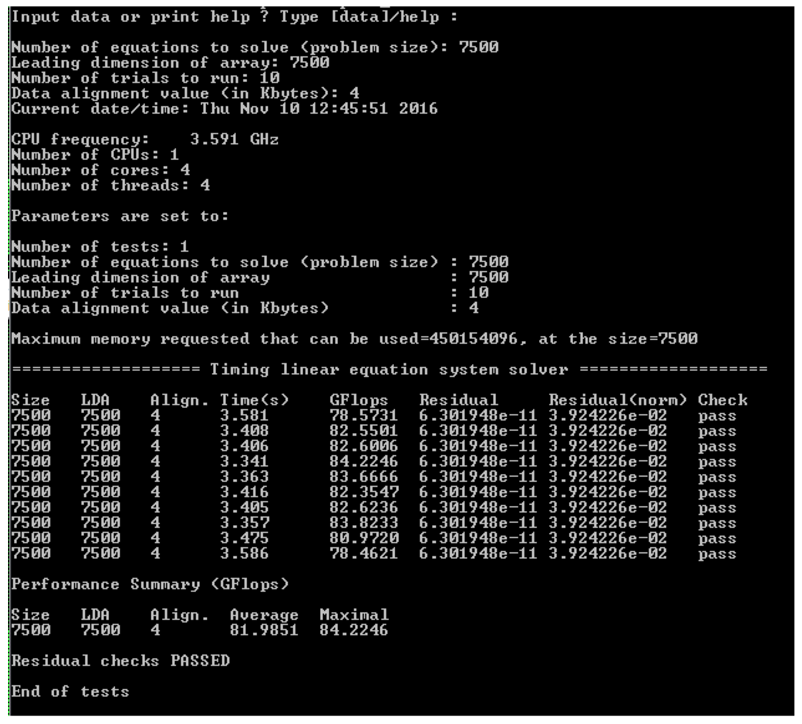
\includegraphics[height=7cm, width=6cm]{linpack_windows.png}
           \end{tabular}
           & \begin{tabular}{l}
             \parbox{0.5\linewidth}{
	     \begin{itemize}
             \item\textbf{Windows 7}
	     \item\textbf{Matrius 7500x7500}
	     \item\textbf{Promig 10 proves}
	     \end{itemize}}
         \end{tabular}  \\
\end{tabular}
}
\frame {
    \frametitle{Comparativa de tiempos/recursos para una aplicación en el mismo PC bajo distintos SO}
    \framesubtitle{Simulació 2 - Linpack Benchmark}

  \begin{tabular}{cl}  
         \begin{tabular}{c}
           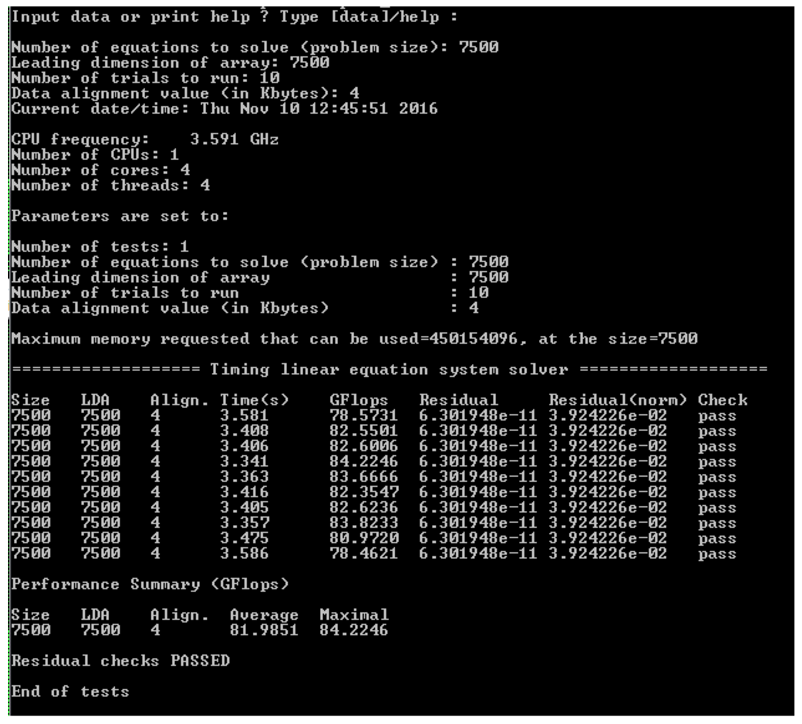
\includegraphics[height=7cm, width=6cm]{linpack_windows.png}
           \end{tabular}
           & \begin{tabular}{l}
             \parbox{0.5\linewidth}{
	     \begin{itemize}
             \item\textbf{openSUSE}
	     \item\textbf{Matrius 7500x7500}
	     \item\textbf{Promig 10 proves}
	     \item\textbf{81.951 GFLOPS}
	     \end{itemize}}
         \end{tabular}  \\
\end{tabular}
}
\frame {
  \frametitle{Comparativa de tiempos/recursos para una aplicación en el mismo PC bajo distintos SO}
  \framesubtitle{Simulació 2 - Linpack Benchmark}
  \begin{itemize}
  \item\textbf{openSUSE}
	  \begin{itemize}
	  \item{86.3305 GFLOPS}
	  \end{itemize}
  \item\textbf{Windows 7}
	  \begin{itemize}
	  \item{81.951 GFLOPS}
	  \end{itemize}
   \end{itemize}
}

\frame {
    \frametitle{Comparativa de tiempos/recursos para una aplicación en el mismo PC bajo distintos SO}
    \framesubtitle{Simulació 3 - Firefox}
    \begin{itemize}
    \item {Sistemes operatius:}
	\begin{itemize}
	\item\textbf{openSUSE 13.2 (Harlequin) (64 bits)}
    	\item\textbf{Windows 7 ENTERPRISE (64 bits)}
    	\end{itemize}
    \item {Medició:}
	\begin{itemize}
	\item\textbf{Firefox}
    	\end{itemize}
    \item {Processador:}
	\begin{itemize}
	\item\textbf{Intel(R) Core(TM) i5-3470 CPU @ 3.20GHz - 64 bits}
    	\end{itemize}
    \item {Memòria RAM:}
	\begin{itemize}
	\item\textbf{8 GB}
    	\end{itemize}
    \item {Nom de l'equip:}
	\begin{itemize}
	\item\textbf{c6s301pc42}
    	\end{itemize}
    \item {Domini:}
	\begin{itemize}
	\item\textbf{FIBSMB}
    	\end{itemize}
    \end{itemize}
}

\frame {
    \frametitle{Comparativa de tiempos/recursos para una aplicación en el mismo PC bajo distintos SO}
    \framesubtitle{Simulació 3 - Firefox}
    \begin{itemize}
    \item\textbf{openSUSE}
   % \begin{lstlisting}[language=bash,caption={bash version}]#!/bin/bashecho "Hello, world!"\end{lstlisting}
    \item\textbf{!/bin/bash
	START="$(($(date +%s%N)/1000000))"
	cd /home/Desktop/ %firefox "http://www.google.com/" &
	./factorial.out
	END="$(($(date +%s%N)/1000000))" 
	TOTAL=$(($END-$START))
	echo "END: "$END "START: "$START "TOTAL: "$TOTAL}
    \end{itemize}
}
\frame {
    \frametitle{Comparativa de tiempos/recursos para una aplicación en el mismo PC bajo distintos SO}
    \framesubtitle{Simulació 3 - Firefox}

  \begin{tabular}{cl}  
         \begin{tabular}{c}
           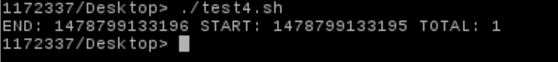
\includegraphics[height=2cm, width=7cm]{firefox_open_suse1.png}
           \end{tabular}
           & \begin{tabular}{l}
             \parbox{0.5\linewidth}{
	     \begin{itemize}
             \item\textbf{openSUSE}
	     \item\textbf{1 Mil·lisegon}
	     \end{itemize}}
         \end{tabular}  \\
\end{tabular}
}
\frame {
    \frametitle{Comparativa de tiempos/recursos para una aplicación en el mismo PC bajo distintos SO}
    \framesubtitle{Simulació 3 - Firefox}
    \begin{itemize}
    \item\textbf{Windows 7}
   % \begin{lstlisting}[language=bash,caption={bash version}]#!/bin/bashecho "Hello, world!"\end{lstlisting}
    \item\textbf{@ECHO OFF
SET START= %time% 
start firefox http://google.com
SET END= %time% 
SET /a TOTAL = %END% - %START%
ECHO END:} %END% START: %START% TOTAL: %TOTAL%}
    \end{itemize}
}
\frame {
    \frametitle{Comparativa de tiempos/recursos para una aplicación en el mismo PC bajo distintos SO}
    \framesubtitle{Simulació 3 - Firefox}

  \begin{tabular}{cl}  
         \begin{tabular}{c}
           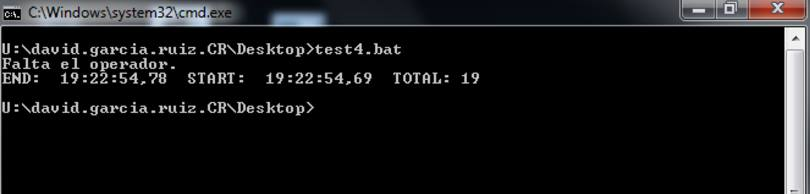
\includegraphics[height=2.5cm, width=7cm]{firefox-windows.png}
           \end{tabular}
           & \begin{tabular}{l}
             \parbox{0.5\linewidth}{
	     \begin{itemize}
             \item\textbf{Windows 7}
	     \item\textbf{19 Mil·lisegons}
	     \end{itemize}}
         \end{tabular}  \\
\end{tabular}
}
\frame {
  \frametitle{Comparativa de tiempos/recursos para una aplicación en el mismo PC bajo distintos SO}
  \framesubtitle{Simulació 3 - Firefox}
  \begin{itemize}
  \item\textbf{openSUSE}
	  \begin{itemize}
	  \item{1 Mil·lisegon}
	  \end{itemize}
  \item\textbf{Windows 7}
	  \begin{itemize}
	  \item{19 Mil·lisegons}
	  \end{itemize}
   \end{itemize}
}
\frame {
  \frametitle{Comparativa de tiempos/recursos para una aplicación en el mismo PC bajo distintos SO}
  \framesubtitle{Conclusions Simulacions}
  \begin{itemize}
  	\item\ No únicament el SO afecta en els temps/recursos
  	\item\ Hi ha \textbf{"Soroll"} que afecta
  	\item\ Identificar que ocasiona "Soroll"
   \end{itemize}
}
\frame {
  \frametitle{Comparativa de tiempos/recursos para una aplicación en el mismo PC bajo distintos SO}
  \framesubtitle{Alternatives millora rendiment SO}
  \begin{itemize}
  	\item\textbf{Windows} 
  	\item\ Pot funcionar més lent del que s'espera
  	\item\ Disc dur més ple del que es recomana
   \end{itemize}
}
\frame {
  \frametitle{Comparativa de tiempos/recursos para una aplicación en el mismo PC bajo distintos SO}
  \framesubtitle{Alternatives millora rendiment SO}
  \begin{itemize}
  	\item\textbf{Windows} 
  	\item\ Tenir més Memòria RAM amb eines com \textbf{ReadyBoost}
  	\item\ Desactivar serveis:
  	\begin{itemize}
            \item Application experience
            \item Computer browser
            \item Security server
  	\end{itemize}
   \end{itemize}
}

\frame {
    \frametitle{Comparativa de tiempos/recursos para una aplicación en el mismo PC bajo distintos SO}
    \framesubtitle{Alternatives millora rendiment SO}

  \begin{tabular}{cl}  
         \begin{tabular}{c}
       %  \begin{figure}
           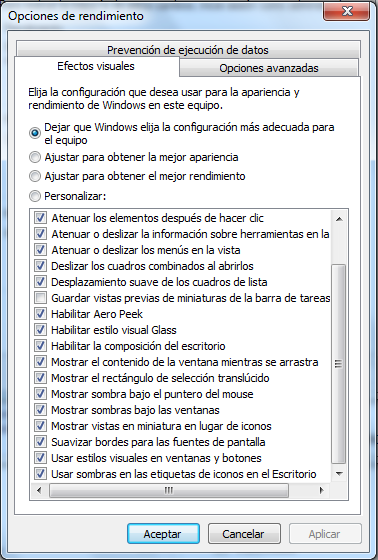
\includegraphics[height=6cm, width=5cm]{efectos_visuales.png}
         %  \caption{Efectos Visuales Windows 7}
        % \end{figure}
           \end{tabular}
           & \begin{tabular}{l}
             \parbox{0.5\linewidth}{
	     \begin{itemize}
             \item{Desactivar efectes visuals}
	     \end{itemize}}
         \end{tabular}  \\
\end{tabular}
}
\frame {
    \frametitle{Comparativa de tiempos/recursos para una aplicación en el mismo PC bajo distintos SO}
    \framesubtitle{Alternatives millora rendiment SO}

  \begin{tabular}{cl}  
         \begin{tabular}{c}
           
\includegraphics[height=3cm, width=2.5cm]{desactivar-uac.png}
         %  \caption{Control de cuentas de usuarios de Windows 7}
           \end{tabular}
           & \begin{tabular}{l}
             \parbox{0.5\linewidth}{
	     \begin{itemize}
             \item{Desactivar UAC \\(Control Cuentas Usuario)}
	     \end{itemize}}
         \end{tabular}  \\
\end{tabular}
}

\frame {
    \frametitle{Comparativa de tiempos/recursos para una aplicación en el mismo PC bajo distintos SO}
    \framesubtitle{Alternatives millora rendiment SO}

  \begin{center} 
    \begin{figure}
           \centering
           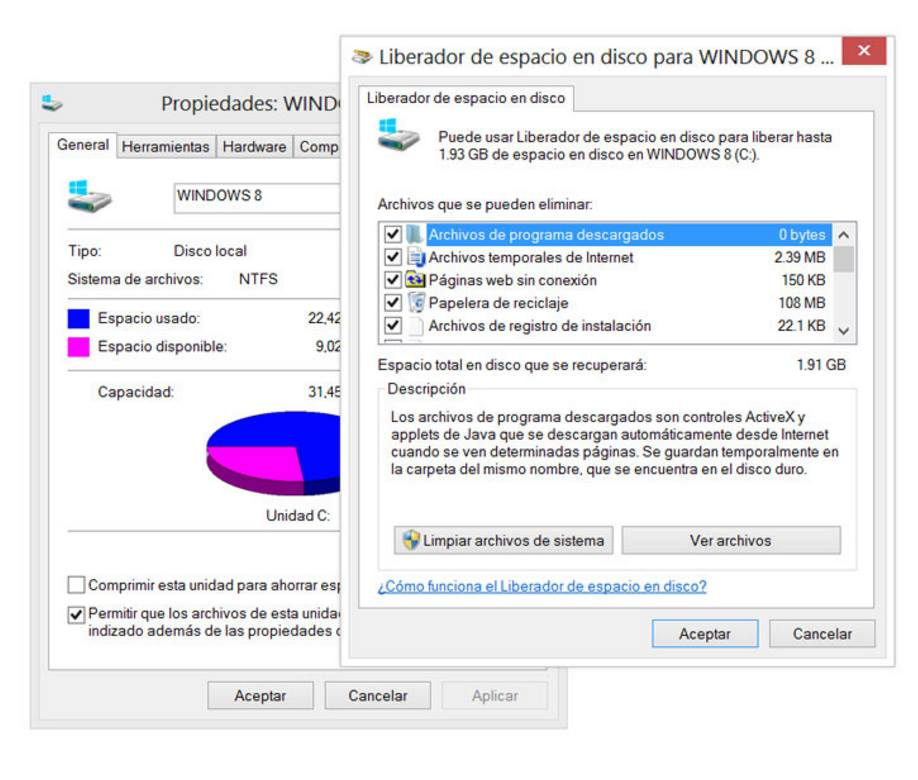
\includegraphics[height=5cm, width=7cm]{liberador-espacio-windows.png}
           \caption{Alliberador d'espai en disc Windows 7}
    \end{figure}
  \end{center}
}
\frame {
    \frametitle{Comparativa de tiempos/recursos para una aplicación en el mismo PC bajo distintos SO}
    \framesubtitle{Alternatives millora rendiment SO}

  \begin{center} 
    \begin{figure}
           \centering
           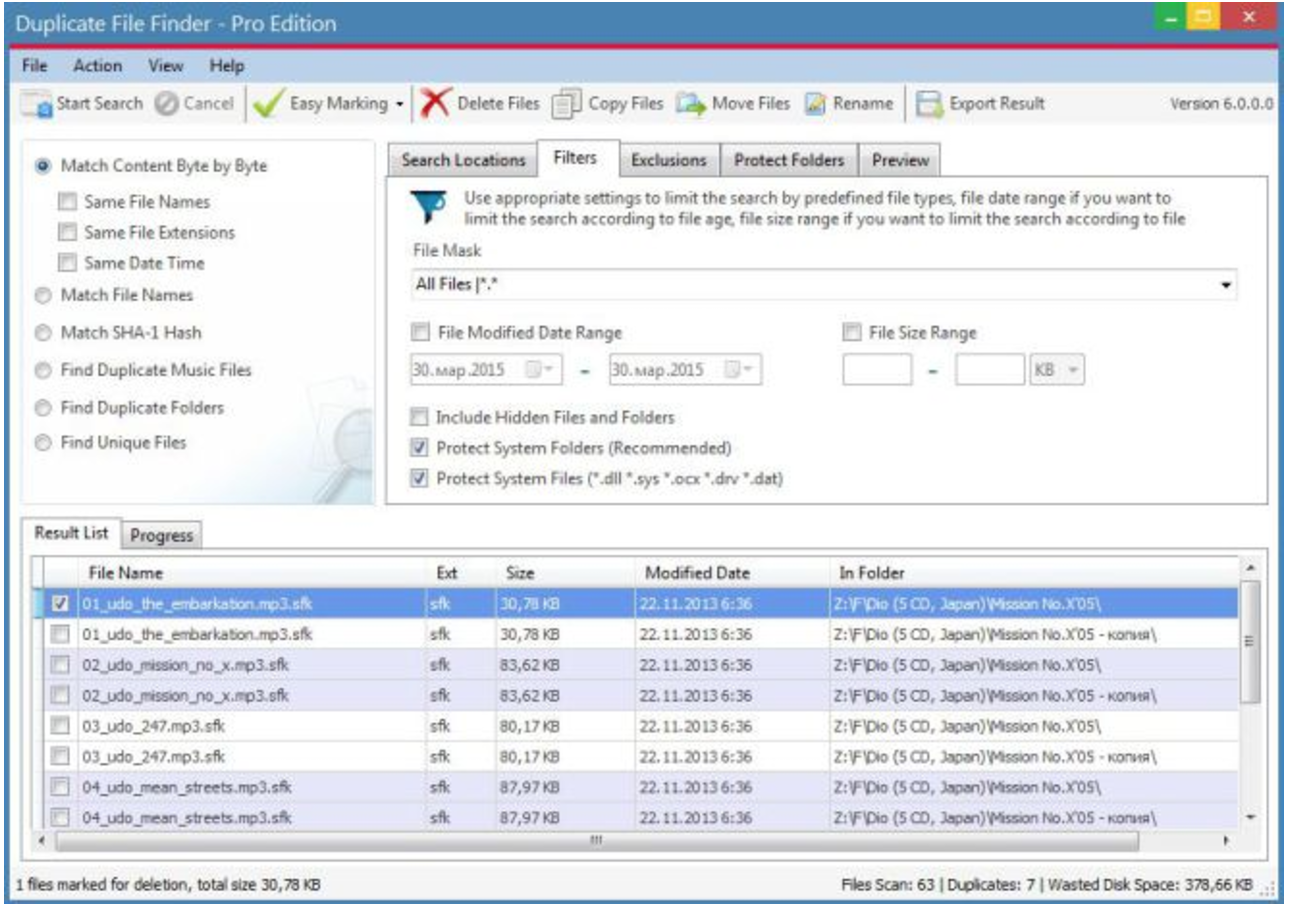
\includegraphics[height=5cm, width=7cm]{duplicate.png}
           \caption{Duplicate File Finder}
    \end{figure}
  \end{center}
}
\frame {
    \frametitle{Comparativa de tiempos/recursos para una aplicación en el mismo PC bajo distintos SO}
    \framesubtitle{Alternatives millora rendiment SO}

  \begin{center} 
    \begin{figure}
           \centering
           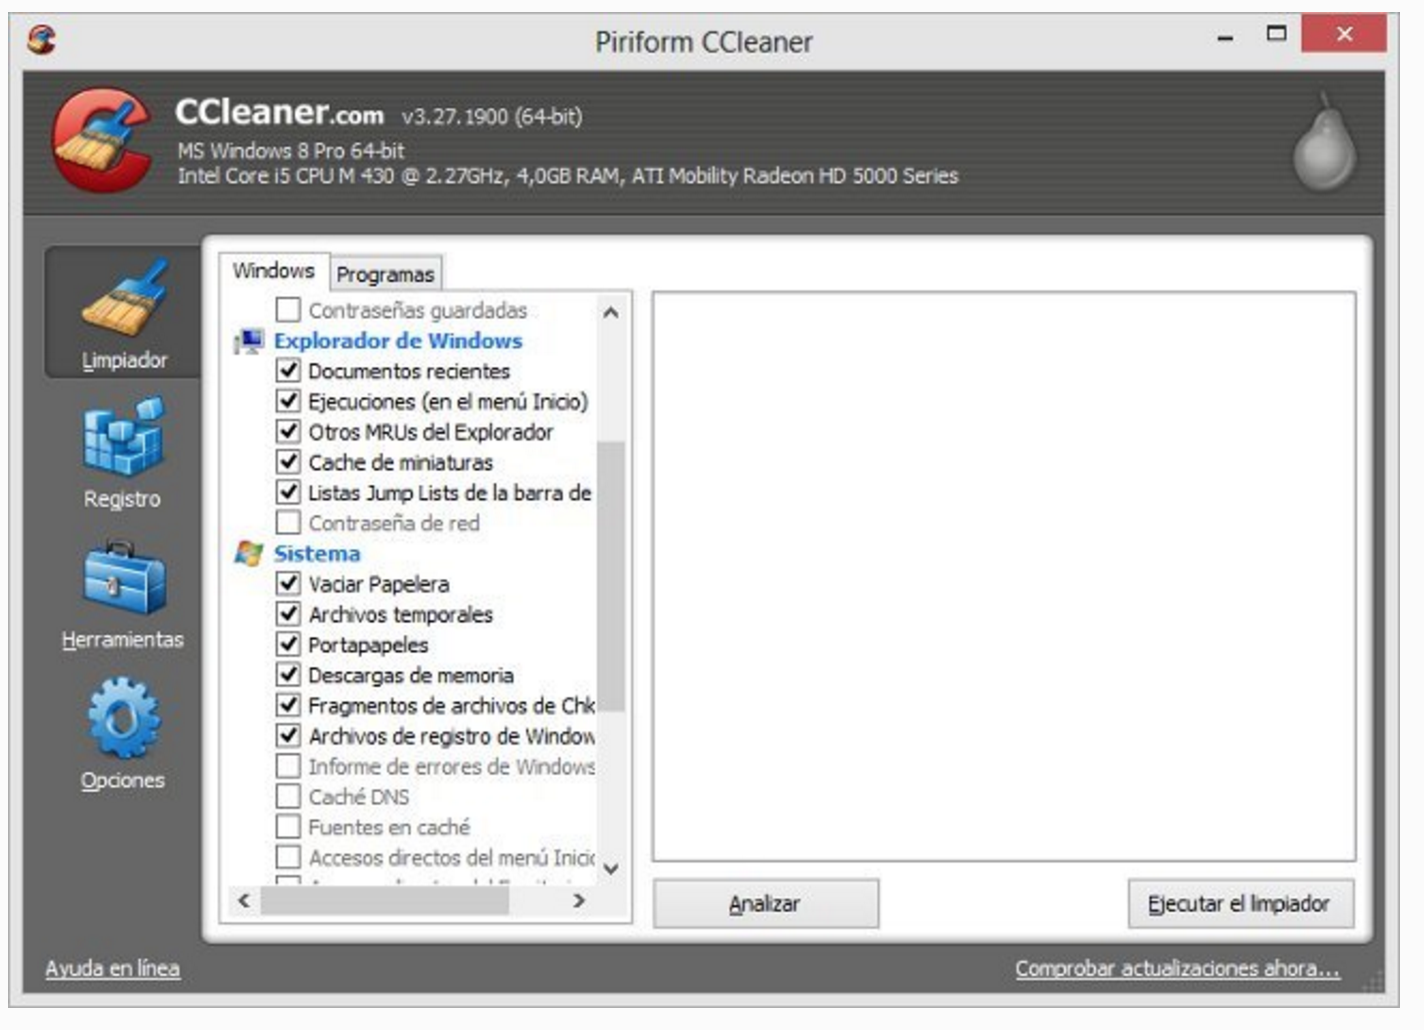
\includegraphics[height=5cm, width=7cm]{ccleaner.png}
           \caption{CCleaner}
    \end{figure}
  \end{center}
}
\frame {
  \frametitle{Comparativa de tiempos/recursos para una aplicación en el mismo PC bajo distintos SO}
  \framesubtitle{Alternatives millora rendiment SO}
  \begin{itemize}
  	\item\textbf{openSUSE} 
  	\item\ Actualitzar el Kernel
  	\item\ Desactivar efectes especials
        \item\ Desinstalar aplicacions no utilitzades 
   \end{itemize}
}
\frame {
    \frametitle{Comparativa de tiempos/recursos para una aplicación en el mismo PC bajo distintos SO}
    \framesubtitle{Alternatives millora rendiment SO}

  \begin{center} 
    \begin{figure}
           \centering
           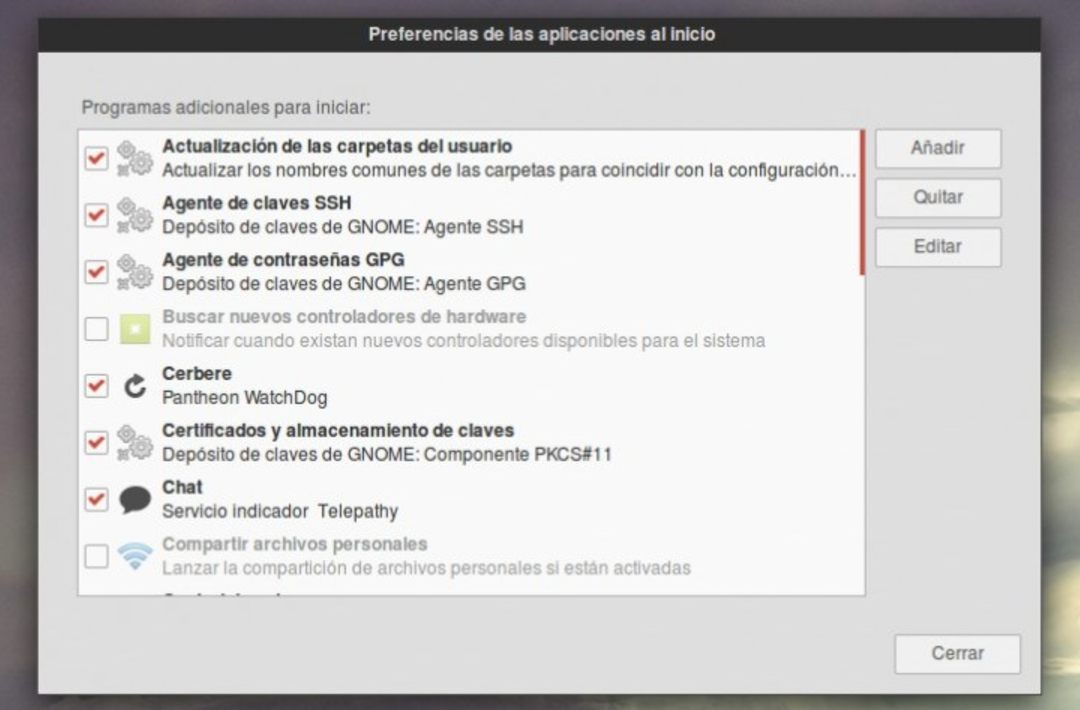
\includegraphics[height=5cm, width=7cm]{desactivar-aplicaciones-linux.png}
           \caption{Preferencias aplicaciones instaladas en Linux}
    \end{figure}
  \end{center}
}
\frame {
    \frametitle{Comparativa de tiempos/recursos para una aplicación en el mismo PC bajo distintos SO}
    \framesubtitle{Alternatives millora rendiment SO}

  \begin{center} 
    \begin{figure}
           \centering
           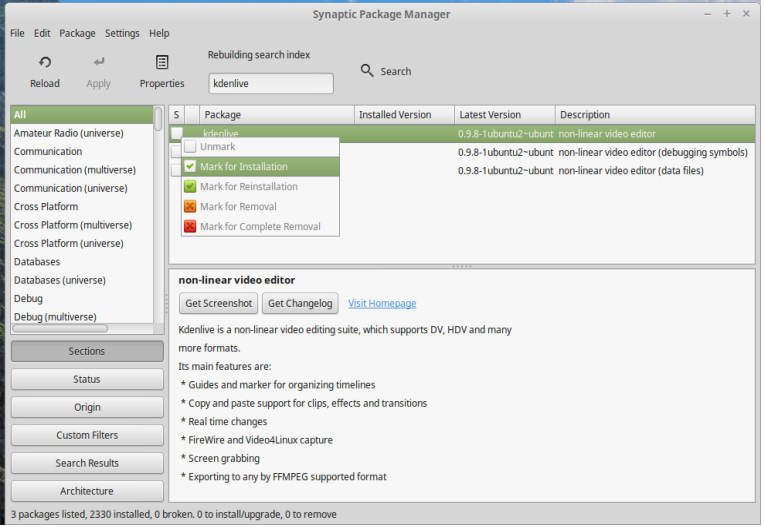
\includegraphics[height=5cm, width=7cm]{limpieza-linux-synaptic.png}
           \caption{Synaptic Package Manager}
    \end{figure}
  \end{center}
}
\frame {
    \frametitle{Comparativa de tiempos/recursos para una aplicación en el mismo PC bajo distintos SO}
    \framesubtitle{Alternatives millora rendiment SO}

  \begin{center} 
    \begin{figure}
           \centering
           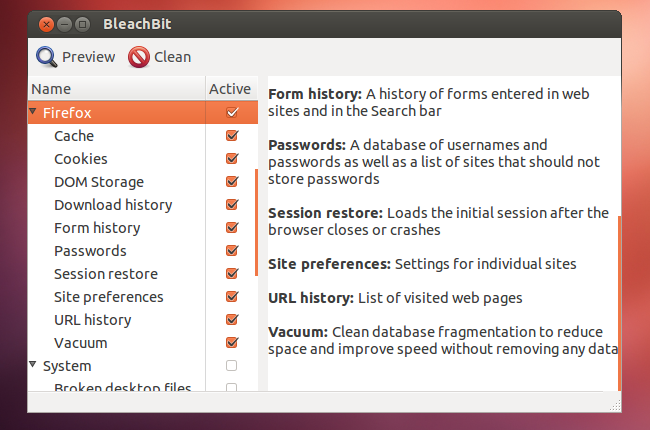
\includegraphics[height=5cm, width=7cm]{limpieza-linux-beatbit.png}
           \caption{BleachBit}
    \end{figure}
  \end{center}
}



% End Arnau Garcia
% Begin Guillem Gordillo

\frame {
    \frametitle{Posibilidades de simulación / virtualización en unos y otros. Interoperabilidad}
    \textbf{Guillem Gordillo}
}

% End Guillem Gordillo

\frame {
    \frametitle{Bibliografía}
    \begin{itemize}
        \item {http://informatica.blogs.uoc.edu/2016/03/08/guia-para-elegir-el-sistema-operativo-de-tu-ordenador-windows-os-x-o-linux/}
        \item {http://www.howtogeek.com/197559/how-to-install-windows-10-on-your-pc/}
        \item {https://help.ubuntu.com/community/Installation}
        \item {https://support.apple.com/en-us/HT204904}
        \item {http://venturebeat.com/2016/03/30/hey-microsoft-how-many-apps-are-in-the-windows-store/}
        \item {https://wiki.ubuntu.com/SoftwareCenter}
    \end{itemize}
}

\end{document}
